% The first official use of the word "Neuroscience" may be in 1962 with Francis O. Schmitt's "Neuroscience Research Program", which was hosted by the Massachusetts Institute of Technology1
% . Therefore, it is not clear who coined the term "neuroscience".

The Neuron. CELL AND MOLECULAR BIOLOGY
IRWIN B. LEVITAN
LEONARD K. KACZMAREK
"how many neurons are involved in the control of a scpecific behavior, where are located and how they are connected. 
All play roles in the output of that circuit. 

Physiologtsts, biochemists, and anatomists  .... Neuroscience is already a mature discipline in its own right. 



Santiago Ramón y Cajal made significant contributions to the field of neuroscience. Here are some of his major contributions:

    Neuron Doctrine: Cajal's greatest contribution to neuroscience is the idea of the "neuron doctrine," which he proposed and supported with evidence. He showed that the nervous system comprises individual cells called neurons, which connect to each other at small, specialized contact zones called synapses. He also demonstrated that a single nerve cell typically possesses three anatomically distinct structures3
    .
    Staining Techniques: Cajal developed staining techniques that allowed him to visualize the structure of the nervous system with exquisite precision. He used these techniques to make many discoveries about the structure and function of neurons1
    .
    Dynamic Polarization: Cajal proposed the Law of Dynamic Polarization, which describes the directional flow of information in the nervous system. According to this law, information flows from the dendrites of a neuron to its cell body and then to its axon6
    .
    Comparative Studies: Cajal conducted extensive comparative studies of the nervous system using material from humans, dogs, cats, rodents, birds, and reptiles. These studies led him to discover novel nuclei and cell types and to reorganize the ideas regarding the connections between neural regions and nuclei6
    .
    Meticulous Artwork: Cajal left behind a vast collection of meticulous and beautiful artwork that captures our understanding of the brain in his time. His drawings are still reproduced in neuroscience textbooks today2
    .

Overall, Cajal's contributions to neuroscience laid the foundations of modern neuroscience and continue to be valuable today.


Neuron- Signalling in the Brain. 
1840, Jacob Schleiden and Theodor Schwann --> Cells definition

Neuron. Three structural elements specific from neurons: axon, dendrites and synapse. 



Adapt models table from
https://www.sciencedirect.com/science/article/pii/S0896627319304441 Figure 2A:
\begin{figure}
    \centering
    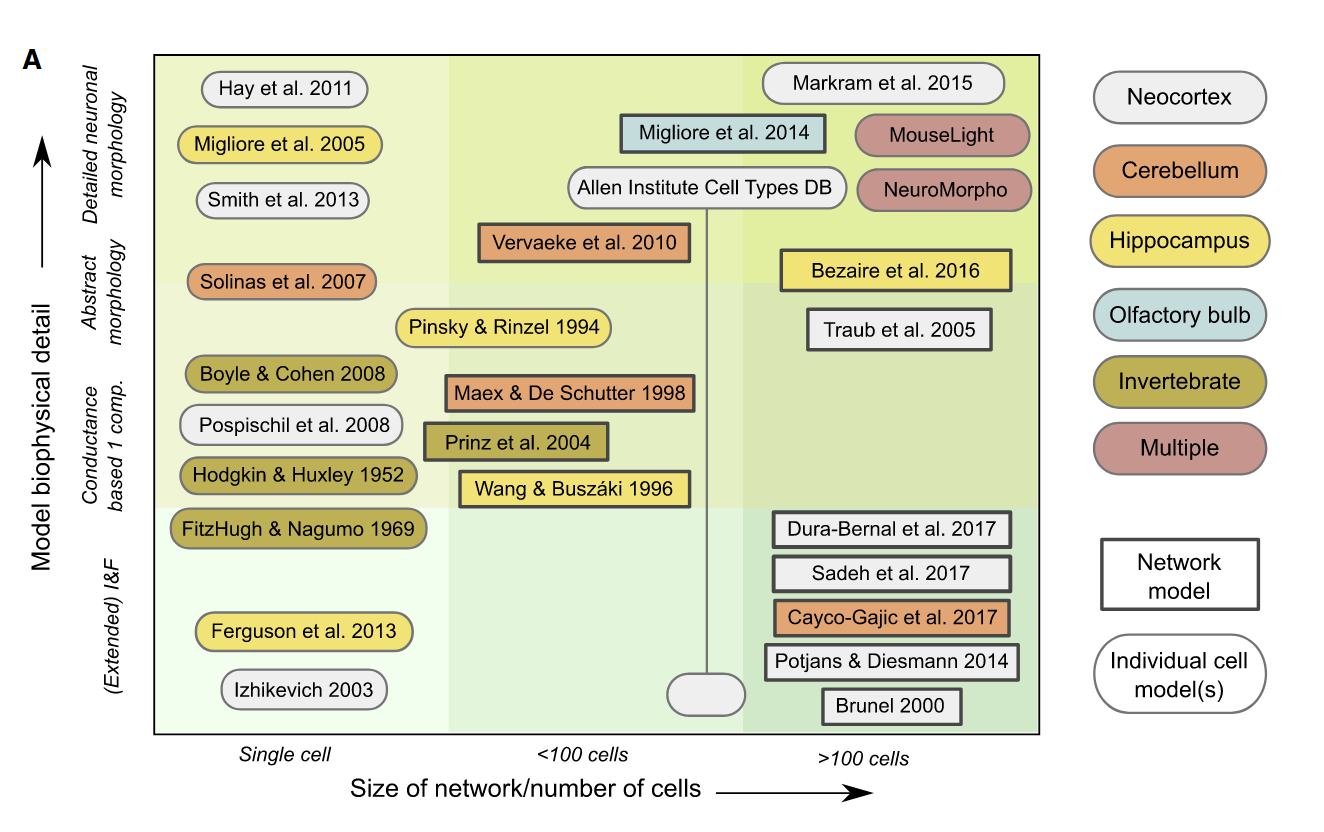
\includegraphics[width=\textwidth]{misc/models-table.png}
    \caption{Caption}
    \label{fig:models-table}
\end{figure}

Lotka-Volterra; Ginsburg-Landau